\usetikzlibrary{decorations.pathreplacing, arrows.meta, calc, positioning}

\chapter{Modello a cascata}
\section{Cosa è?}
Il modello a cascata rappresenta storicamente il primo approccio sistematico e disciplinato allo sviluppo del software.

È un modello di processo lineare e sequenziale, dove lo sviluppo scorre verso il basso attraverso diverse fasi, proprio come l'acqua di una cascata.

In questo approccio, ogni fase deve essere completata e approvata prima di poter passare a quella successiva, rendendo difficile tornare indietro

\section{Le fasi del modello}
Le fasi tipiche sono organizzate in ordine rigoroso

\begin{figure}[H]
    \centering
    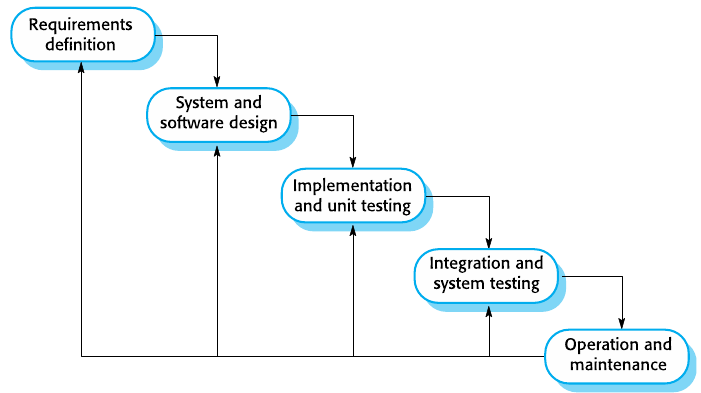
\includegraphics[width=0.6\textwidth]{Immagini/Schermata_20260707_122604.png}
\end{figure}

\subsection{Analisi dei Requisiti}
In questa fase iniziale, tutto ciò che il sistema che deve fare viene identificato, documentato e "congelato".

Il risultato è un documento dettagliato di specifica dei requisiti che funge da contratto tra cliente e sviluppatori

\subsection{Progettazione}
Si definisce l'architettura del sistema, le strutture dati, le interfacce e i diagrammi di design.

L'obiettivo è trasformare i requisiti in un piano tecnico solido

\subsection{implementazione}
Gli sviluppatori scrivono il codice.

Il lavoro è focalizzato sulla traduzione del design in software funzionante, spesso lavorando su moduli o unità separate

\subsection{Collaudo}
I componenti vengono integrati e il sistema viene testato nella sua interezza per verificare che rispetti le specifiche definite nella prima fase

\subsection{Rilascio e Manutenzione}
Il sistema viene messo in produzione (distribuito agli utenti).

La fase di manutenzione riguarda la correzione di errori scoperti dopo il rilascio o l'adattamento del sistema a nuovi requisiti ambientali

\section{Caratteristiche chiave}
\subsection{Plan-driven}
L'enfasi è posta sulla pianificazione dettagliata e sulla documentazione.

Il progresso è misurato attraverso il complemento di fasi e artefatti documentali

\subsection{Specializzazione}
Spesso, fasi diverse sono assegnate a team diversi

\subsection{Rigidità}
Una volta che si è superata una fase, non si dovrebbe tornare indietro.

Se emergono problemi, il modello non prevede meccanismi nativi per gestire il cambiamento, se non ricominciando il ciclo da capo


\section{Vantaggi}
\subsection{Semplicità e chiarezza}
È estremamente semplice da gestire.

Le scadenze, i budget e i progressi sono facili da visualizzare su un diagramma di Gantt

\subsection{Ideale per requisiti stabili}
È efficace in progetti dove i requisiti sono ben compresi fin dall'inizio e non cambieranno mai


\section{Svantaggi}
\subsection{Incapacità di gestire i cambiamenti}
Nel mondo reale, i clienti raramente sanno cosa vogliono finchè non vedono il software.

Se i requisiti cambiano a metà percorso, i costi di modifica diventano proibitivi

\subsection{Feedback tardivo}
Il cliente vede il software funzionante solo nelle fasi finali del progetto.

Se si accorge che il prodotto non è quello desiderato, il danno economico e temporale è irreparabile

\subsection{Debito di integrazione}
Poichè il test avviene solo alla fine, eventuali errori architetturali o di comunicazione tra i moduli emergono tardi, rendendo la loro correzione estremamente complessa


\chapter{UP - Unified Process}
\section{Cosa è?}
Il Processo Unificato è un framework di processo iterativo ed evolutivo ampiamente utilizzato nell'ingegneria del software, specificamente concepito per lo sviluppo di sistemi orietanti agli oggetti.

\section{Le 3 caratteristiche fondamentali dell'UP}
Tutto lo sviluppo all'interno del framework UP è guidato da 3 caratteristiche essenziali

\subsection{Pilotato dai casi d'uso}
Lo sviluppo è interamente guidato dalle reali necessità degli utenti finali.

I casi d'uso vengono utilizzati per definire i requisiti, pianificare le iterazioni, guidare la progettazione e strutturare i test, garantendo un coinvolgimento continuo degli utenti per raccogliere feedback

\subsection{Guidato dai fattori di rischio}
Il team non sviluppa le funzionalità in modo casuale o sequenziale, ma affronta e risolve fin dalle primisse iterazioni le problematiche a maggior rischio tecnico o a più alto valore aziendale

\subsection{Incentrato sull'architettura}
Piuttosto che concentrarsi immediatamente sui dettagli secondari, le fasi iniziali miriano a costruire, testare e stabilizzare un nucleo architettonico solido e coeso

\section{Le 4 fasi del cilcio di vita}
Un progetto gestito con UP organizza il proprio asse temporale suddividendo in 4 macro-fasi sequenziali.

Al termine di ciascuna fase è prevista un "milestone", ovvero un momento in cui si verifica una decisione o valutazione significativa per stabilere se procedere.

\begin{center}
    \begin{tikzpicture}[font=\sffamily, scale=0.75, transform shape]
    % ==========================================
    % PARAMETRI GEOMETRICI
    % ==========================================
    \def\w{1.3}    % Larghezza di una singola iterazione
    \def\h{1.5}    % Altezza della faccia frontale dei blocchi
    \def\dx{0.25}  % Profondità 3D (offset asse X)
    \def\dy{0.35}  % Profondità 3D (offset asse Y)

    % Coordinate X di inizio per ogni fase (calcolate con larghezza 1.3 e un gap di 0.15)
    \def\xIdeaz{0}
    \def\xElab{1.45}
    \def\xCostr{4.20}
    \def\xTrans{12.15}
    
    % ==========================================
    % MACRO PER DISEGNARE I BLOCCHI 3D DELLE FASI
    % #1 = coordinata X iniziale
    % #2 = numero di iterazioni (sottoblocchi)
    % #3 = testo della fase
    % ==========================================
    \newcommand{\drawphase}[3]{
        \pgfmathsetmacro{\totalw}{#2 * \w}
        
        % Faccia laterale destra (disegnata per prima per la sovrapposizione)
        \draw [fill=gray!20] 
            (#1+\totalw, 0) -- 
            (#1+\totalw+\dx, \dy) -- 
            (#1+\totalw+\dx, \h+\dy) -- 
            (#1+\totalw, \h) -- cycle;
            
        % Faccia superiore
        \draw [fill=gray!10] 
            (#1, \h) -- 
            (#1+\dx, \h+\dy) -- 
            (#1+\totalw+\dx, \h+\dy) -- 
            (#1+\totalw, \h) -- cycle;
            
        % Faccia frontale
        \draw [fill=white] (#1, 0) rectangle (#1+\totalw, \h);
        
        % Linee interne per dividere le iterazioni
        \foreach \i in {1,...,#2} {
            \ifnum\i<#2
                \draw (#1+\i*\w, 0) -- (#1+\i*\w, \h);
                \draw (#1+\i*\w, \h) -- (#1+\i*\w+\dx, \h+\dy);
            \fi
        }
        
        % Etichetta testuale al centro del blocco frontale
        \node at (#1+\totalw/2, \h/2) {\textit{#3}};
    }

    % ==========================================
    % DISEGNO DELLE 4 FASI
    % ==========================================
    \drawphase{\xIdeaz}{1}{ideaz.}
    \drawphase{\xElab}{2}{elaborazione}
    \drawphase{\xCostr}{6}{costruzione}
    \drawphase{\xTrans}{2}{transizione}

    % ==========================================
    % PARENTESI GRAFFE SUPERIORI
    % ==========================================
    % Parentesi "iterazione" (sopra il primo blocco di elaborazione)
    \draw [decorate, decoration={brace, amplitude=5pt}] 
        (\xElab+\dx, 2.2) -- (\xElab+\w+\dx, 2.2) 
        node[midway, above=6pt] {\small \textit{iterazione}};

    % Parentesi "fase" (sopra tutta la costruzione)
    \draw [decorate, decoration={brace, amplitude=6pt}] 
        (\xCostr+\dx, 2.2) -- (\xCostr+6*\w+\dx, 2.2) 
        node[midway, above=7pt] {\small \textit{fase}};

    % Parentesi "ciclo di sviluppo" (sopra tutto il diagramma)
    \draw [decorate, decoration={brace, amplitude=8pt}] 
        (\xIdeaz+\dx, 3.2) -- (\xTrans+2*\w+\dx, 3.2) 
        node[midway, above=10pt] {\textit{ciclo di sviluppo}};


    % ==========================================
    % FRECCE E TESTI INFERIORI
    % ==========================================
    
    % Milestone (punta al gap tra elaborazione e costruzione)
    \def\xMilestone{4.125}
    \draw [-Latex] (\xMilestone, -1.0) -- (\xMilestone, -0.1);
    \node [anchor=north, align=left, text width=3.4cm] at (\xMilestone, -1.2) {
        \textit{milestone}\\[0.5em]
        \small La fine di un'iterazione in cui si verifica una decisione o una valutazione significativa.
    };

    % Release (punta al centro della costruzione)
    \def\xRelease{8.1}
    \draw [-Latex] (\xRelease, -1.0) -- (\xRelease, -0.1);
    \node [anchor=north, align=left, text width=3.6cm] at (\xRelease, -1.2) {
        \textit{release}\\[0.5em]
        \small Un sottoinsieme stabile ed eseguibile del prodotto finale. La fine di ogni iterazione produce una release minore.
    };

    % Incremento (testo senza freccia posizionato tra costruzione e transizione)
    \def\xIncremento{11.3}
    \node [anchor=north, align=left, text width=3.3cm] at (\xIncremento, -1.2) {
        \textit{incremento}\\[0.5em]
        \small La differenza (delta) tra le release di 2 iterazioni successive.
    };

    % Release produzione finale (punta alla fine della transizione)
    \def\xFinale{14.75}
    \draw [-Latex] (\xFinale, -1.0) -- (\xFinale, -0.1);
    \node [anchor=north, align=left, text width=3.4cm] at (\xFinale, -1.2) {
        \textit{release produzione finale}\\[0.5em]
        \small A questo punto il sistema viene rilasciato e consegnato ai clienti.
    };

\end{tikzpicture}
\end{center}

\subsection{Ideazione}
Costituisce l'avvio formale del progetto.

L'obiettivo principale non è programmare, ma valutare la fattibilità. In questa fase si definisce una visione approssimativa, si valuta la portata(scope), si individuano i casi d'uso principali e si abbozzano stime preliminari di costi e tempi

\subsection{Elaborazione}
È la fase più critica, incentra sulla realizzazione e sul test iterativo del nucleo dell'architettura.

Qui si mitigano i rischi maggiori, si definisce la maggior parte dei requisiti e si formulano stime molto realistiche su budget e tempistiche

\subsection{Costruzione}
È la fase dedicata alla produzione intensiva.

Vengono sviluppati iterativamente tutti gli elementi rimanenti, che sono tipicamente i più facili e a minor rischio, preparando il sistema per la capacità operative iniziali

\subsection{Transizione}
Ha lo scopo di portare il software agli utenti finali.

Include attività come il beta testing, la correzione degli ultimi difetti e si conclude con la consegna del prodotto finale pronto per la produzione

\section{Dinamica di Sviluppo: Iterazioni, Discipline e incrementi}
Nell'UP, il lavoro non procede in modo lineare con blocchi monolitici di tempo, ma attraverso cicli più agili

\subsection{Iterazioni}
Il tempo è ripartito in iterazioni brevi e con una durata prefissata(timeboxed).

Ogni iterazione è un "mini-progetto" autonomo che include attività(o discipline) di pianificazione, analisi dei requisiti, progettazione, costruzione del codice, integrazione e test

\subsection{Variazione dell'impegno}
Sebbene ogni iterazione possa comprendere tutte le discipline, l'enfasi e l'impegno relativo cambiano a seconda della fase in cui ci si trova.

\subsection{Release e incremento}
Ogni iterazione termina con la produzione di una release, ovvero un sottoinsieme stabile ed eseguibile del prodotto finale.

La differenza funzionale tra due release successive prende il nome di incremento.

Questo processo permette al sistema di evolvere e convergere gradualmente verso la soddisfazione dei requisiti corretti

\section{Vantaggi}
Garantisce un'estrema flessibilità, consentendo di adattare il processo eliminando la burocrazia.

Assicura la mitigazione precoce dei rischi strutturali durante l'elaborazione e, producendo software eseguibile a ogni iterazione, permette di ottenere progressi tangibili e un feedback continuo dagli utenti

\section{Svantaggi}
Per i manager legati a visioni tradizionali, il focus sul software funzionanete rispetto alla documentazione massiva può trasmettere un senso di scarsa visibilità burocratica.

Inoltre, crescendo per continui incrementi, la struttura del software tende a degradarsi nel tempo(Debito Tecnico), richiedendo investimenti costanti in refactoring.

Infine esiste il grave rischio di "cattiva interpretazione": se si cerca di definre tutti i requisiti e l'architettura in dettaglio prima di programmare, l'UP fallsice, trasformandosi in un finto e rigido modello a cascata

\chapter{Agile}
\section{Cosa è?}
Agile non è un singolo processo rigido, ma piuttosto un termine ombrello che indica una forma di sviluppo iterativo orientata a incoraggiare una risposta rapida e flessibile ai cambiamenti.

All'interno di questa famiglia, il framework più famoso e utilizzato per organizzare il lavoro è Scrum, che ha lo scopo di rilasciare software con il più alto valore nel minor tempo possibile

\section{Valori e Principi}
Agile si fonda su un manifesto valoriale nato nel 2001.

I quattro valori fondamentali affermano che, pur riconoscendo l'importanza degli elementi a destra, si attribuisce più valore a quelli a sinistra:
\begin{itemize}
    \item Gli individui e le interazioni contano più dei processi e degli strumenti
    \item Il software funzionante è più importante della documentazione esaustiva
    \item La collaborazione con il cliente supera la negoziazione dei contratti
    \item Rispondere al cambiamento è più vitale che seguire perdissequamente un piano
\end{itemize}

\section{Flusso di valoro: Sprint e Artefatti}
La pianificazione Agile è puramente incrementale.

Si basa su cicli di vita brebe in cui si alternano continuamente specifica, sviluppo e validazione

\subsection{Product Backlog}
È il "serbatoio" di tutto il lavoro.

Consiste in un elenco delle cose da fare:
\begin{itemize}
    \item funzionalità
    \item requisiti
    \item storie utente 
    \item task tecnici
\end{itemize}

\subsection{Spint (iterazione)}
È il cuore pulsante del processo.

Si tratta un'iterazione di sviluppo con una durata prefissata (timeboxing), solitamente compresa tra le 2 e le 4 settimane

\subsection{Daily Scrum}
Un incontro quotidiano in cui il team esamina i progressi fatti nelle ultime 24 ore e definisce le priorità della giornata in corso

\subsection{Incremento Potenzialmente Rilasciabile}
Alla fine di ogni Sprint, il team deve fornire un incremento di software finito,

L'idea è che debba essere pronto per la produzione, senza richiedere ulteriori cilci di test esterni

\subsection{Velocity}
È una metrica fondamentale che stima quanto lavoro il team riesce a smaltire in un singolo Sprint.

Serve per calibrare i carichi di lavoro futuri in base alle reali prestazioni.

\section{Vantaggi}
La pianificazione incrementale rende estremamente facile modificare il processo per riflettere le mutevoli esigenze dei clienti, un requisito fondamentale poichè pochi sistemi aziendali hanno requisiti stabili.

Le consenge continue promuovo la visibilità, la motivazione del team e la soddisfazione del cliente

\section{Svantaggi}
L'assunto che l'incremento di fine Sprint sia sempre "potenzialmente rilasciabile" in pratica non è sempre realizzabile.

Inoltre, richiedendo team piccoli e auto-organizzati, scala con molta difficoltà su progetti enormi in cui un sistema viene sviluppato in siti distribuiti

\chapter{SCRUM}
\section{Cosa è?}
Mentre Agile è la "filosofia" di base, Scrum è l'implementazione pratica: un framework iterativo e incrementale progettato per sviluppare e rilasciare prodotti complessi massimizzando il valore nel minor tempo possibile.

\section{Ruoli in Scrum}
A differenza dei modelli tradizionali che prevedono decine di figure gerarchiche, Scrum semplifica l'organizzazione in 3 ruole fondamentali eliminando le figure di project management classiche

\subsection{Product Owner}
È un individuo che rappresenta la voce del business e del cliente.

Il suo compito è identificare le caratteristiche e i requisiti del prodotto, assegnare loro le priorità per lo sviluppo e revisionare continuamente la lista delle cose da fare.

Assicura che il progetto continui a soddisfare le esigenze critiche di business

\subsection{Team di Sviluppo}
Un gruppo auto-organizzato di sviluppatori.

Una regola d'oro di Scrum è che questo team non dovrebbe superare le 7 persone.

Sono responsabili in autonomia dello sviluppo tecnico del software e della stesura dei documenti essenziali del progetto.

Nessuno dice al team come trasformare i requisiti in software funzionante

\subsection{ScrumMaster}
È il "facilitatore" del processo.

Il suo scopo è garantire che il team comprenda e applichi correttamente la teoria e le pratiche di Scrum, rimuovendo gli ostacoli esterni che protrebbe rallentare il Team di Sviluppo

\section{Elaborati}
Scrum riduce al minimo la documentazione burocratica, concentrandosi su 3 "artefatti" principali che garantiscono trasparenza e ispezione

\subsection{Product Backlog}
È l'elenco dinamico e prioritizzato di tutto il lavoro "da fare".

Può contenere definizioni di nuove funzionalità, requisiti software, storie utente, correzioni di bug o descrizioni di compiti supplementari.

È gestito unicamente dal Product Owner

\subsection{Sprint Backlog}
È il sottoinsieme di elementi del Product Backlog che il Team di Sviluppo seleziona per essere completato nell'iterazione corrente, unito al piano tecnico per realizzarli

\subsection{Incremento Potenzialmente Rilasciabile}
È l'output fondamentale alla fine di ogni iterazione.

Significa che il software prodotto dove trovarsi in uno stato "finito" e non dovrebbe richiedere ulteriore lavoro per essere incorporato nel prodotto finale

\section{Ciclo di vita}
Il lavoro in Scrum non procede per lunghe fasi monolitiche, ma attraverso cicli fissi

\subsection{Sprint}
È il cuore di Scrum, un'iterazione temporale prefissata (timebox), solitamente di 2, 3 o 4 settimane. Durante lo Sprint il team lavora ininterrottamente per trasformare parte del Product Backlog in un Incremento Potenzialmente Rilasciabile

\subsection{Velocity}
È una metrica fondamentale usata in Scrum per misurare quanto lavoro (es. quanti "punti" o requisiti) il team riesce effettivamente a smaltire in un singolo Sprint. Non serve per mettere pressione, ma per calibrare e pianificare realisticamente i carichi di lavoro degli Sprint futuri in base alle prestazioni reali

\subsection{Eventi chiave}
All'interno dello Sprint avvengono eventi fissi come:
\begin{enumerate}
    \item Sprint Planning
    \item Daily Scrum un allineamento quotidiano di 15 minuti del team di sviluppo
    \item Sprint Review per mostrare l'incremento al cliente
    \item Sprint Retrospective per migliorare il processo stesso
\end{enumerate}

\section{Vantaggi}
\subsection{flessibilità e Adattabilità}
La pianificazione incrementale rende estremamente facile modificare il processo per riflettere le mutevoli esigenze dei clienti.

Questo è vitale, poichè pochissimi sistemi aziendali hanno requisiti stabili fin dall'inizio

\subsection{Motivazione e Visibilità}
Le consegne continue promuovono un'alta visibilità sui progessi, aumentando la motivazione del team e la soddisfazione del cliente

\section{Svantaggi}
\subsection{Il mito dell'incremento "Shippable"}
L'assunto che l'incremento di fine Sprint sia sempre pronto per la produzione, senza richiedere ulteriori cicli di test o integrazione di sistema, in pratica non è sempre realizzabile

\subsection{Problemi di scalabilità}
Richiedendo team molto piccoli (max 7 persone), coesi e auto-organizzati, Scrum puro scala con molta difficoltà su progetti enormi in cui lo sviluppo è distribuito in diverse sedi mondiali o richiede centinaia di sviluppatori. In questi casi, i modelli "guidati dal piano" (o framework scalati ibridi) funzionano spesso meglio